\PassOptionsToPackage{svgnames, table}{xcolor}
\documentclass[8pt]{extarticle}

\usepackage{mcs_style}

\begin{document}
    
    \fullwidthheader{MATLAB\,\,CHEAT\,\,SHEET}
    
    \begin{center}
        \vspace*{0.5cm}
        {\Large\bfseries Throughout this document $x$ and $y$ will be either row or column vectors and $A$ will always be a matrix.}
    \end{center}
    
    \begin{multicols}{2}
        \centering
        
        % -------------------------------------------------------
        % Basics
        % -------------------------------------------------------
        \begin{fancytable}{Basics}
            \texttt{clc} & Clear command window\\
            \texttt{clear} & Clear all variables\\
            \texttt{clf} & Clear all plots\\
            \texttt{close all} & Close all plots\\
            \texttt{doc function} & Open help page for function\\
            \texttt{\% This is a comment} & Comments\\
            \texttt{ctrl-c} & Abort the current operation\\
            \texttt{format short} & Display 4 decimal places\\
            \texttt{format long} & Display 15 decimal places\\
            \texttt{disp('text')} & Print text\\ \chline{Header}
        \end{fancytable}
        
        % -------------------------------------------------------
        % Defining/Changing Variables
        % -------------------------------------------------------
        \begin{fancytable}{Defining and Changing Variables}
            \texttt{a = 3} & Define variable $a$ to be $3$\\
            \texttt{x = [1, 2, 3]} & Set $x$ to be the row vector $[1, 2, 3]$\\
            \texttt{x = [1; 2; 3]} & Set $x$ to be the column vector $[1, 2, 3]^T$\\
            \texttt{A = [1, 2, 3, 4;} & Set $A$ to be a $3 \times 4$ matrix \\
            \rowcolor{row1!75}\qquad\,\,\,\texttt{5, 6, 7, 8;} & \\
            \qquad\,\,\,\texttt{9, 10, 11, 12]} & \\
            \texttt{x(2) = 7} & Change $x$ from $[1, 2, 3]$ to $[1, 7, 3]$\\
            \texttt{A(2,1) = 0} & Change $A_{2,1}$ from $5$ to $0$ \\ \chline{Header}
        \end{fancytable}
        
        % -------------------------------------------------------
        % Basic Arithmetic and Functions
        % -------------------------------------------------------
        \begin{fancytable}{Basic Arithmetic and Functions}
            \texttt{3*4}, \texttt{7+4}, \texttt{2-6}, \texttt{8/3} & multiply, add, subtract and divide\\
            \verb+3^7+ & Compute $3^7$\\
            \texttt{sqrt(5)} & Compute $\sqrt{5}$\\
            \texttt{log(3)} & Compute $\ln(3)$\\
            \texttt{log10(100)} & Compute $\log_{10}(100)$\\
            \texttt{abs(-5)} &  Compute $|-5|$\\
            \texttt{sin(5*pi/3)} & Compute $\sin(5\pi/3)$\\
            \texttt{floor(3.8)} & Compute $\left \lfloor 3.8 \right \rfloor$\\ \chline{Header}
        \end{fancytable}
        
        % -------------------------------------------------------
        % Constructing Matrices/Vectors
        % -------------------------------------------------------
        \begin{fancytable}{Constructing Matrices and Vectors}
            \texttt{zeros(12, 5)} & Make a $12 \times 5$ matrix of zeros\\
            \texttt{ones(12, 5)} & Make a $12 \times 5$ matrix of ones\\
            \texttt{eye(5)} & Make a $5 \times 5$ identity matrix\\
            \texttt{eye(12, 5)} & Make a $12 \times 5$ identity matrix\\
            \texttt{linspace(1.4, 6.3, 1004)} & Make a vector with $1004$ elements evenly spaced between $1.4$ and $6.3$\\
            \texttt{logspace(1.4, 6.3, 1004)} & Make a vector with $1004$ elements where the log of the spacing is evenly increasing between $1.4$ and $6.3$\\
            \texttt{7:15} & Row vector of $7,\,8,\ldots,14,\,15$ \\ \chline{Header}
        \end{fancytable}
        
        % -------------------------------------------------------
        % Operations on Matrices/Vectors
        % -------------------------------------------------------
        \begin{fancytable}{Operations on Matrices and Vectors}
            \texttt{3 * x} & Multiply every element of $x$ by $3$\\
            \texttt{x + 2} & Add $2$ to every element of $x$\\
            \texttt{x + y} & Element-wise addition of two vectors $x$ and $y$\\
            \texttt{A * y} & Product of a matrix and vector\\
            \texttt{A * B} & Product of two matrices\\
            \texttt{A .* B} & Element-wise product of two matrices\\
            \verb+A ^ 3+ & Square matrix $A$ to the third power\\
            \verb+A .^ 3+ & Every element of $A$ to the third power\\
            \texttt{cos(A)} & Compute the cosine of every element of $A$\\
            \texttt{abs(A)} & Compute the absolute values of every element of $A$\\
            \texttt{A'} & Transpose of $A$\\
            \texttt{inv(A)} & Compute the inverse of $A$\\
            \texttt{det(A)} & Compute the determinant of $A$\\
            \texttt{eig(A)} & Compute the eigenvalues of $A$\\
            \texttt{size(A)} & Get the size of $A$ \\ \chline{Header}
        \end{fancytable}
        
        % -------------------------------------------------------
        % Portions of Matrices/Vectors
        % -------------------------------------------------------
        \begin{fancytable}{Entries of Matrices and Vectors}
            \texttt{x(2:12)} & The \nth{2} to the \nth{12} elements of $x$\\
            \texttt{x(2:end)} & The \nth{2} to the last elements of $x$\\
            \texttt{x(1:3:end)} & Every third element of $x$ from the first to last\\
            \texttt{A(5,:)} & Get the \nth{5} row of $A$\\
            \texttt{A(:,5)} & Get the \nth{5} column of $A$\\
            \texttt{A(5, 1:3)} & Get the first to third elements in the \nth{5} row\\ \chline{Header}
        \end{fancytable}
        
        % -------------------------------------------------------
        % Plotting
        % -------------------------------------------------------
        \begin{fancytable}{Plotting}
            \texttt{plot(x,y)} & Plot $y$ versus $x$ (must be the same length)\\
            \texttt{loglog(x,y)} & Plot $y$ versus $x$ on a log-log scale (both axes have a logarithmic scale)\\
            \texttt{semilogx(x, y)} & Plot $y$ versus $x$ with $x$ on a log scale\\
            \texttt{semilogy(x, y)} & Plot $y$ versus $x$ with $y$ on a log scale\\
            \texttt{axis equal} & Force the $x$ and $y$ axes to be scaled equally\\
            \texttt{title('A Title')} & Add a title to the plot\\
            \texttt{xlabel('x label')} & Add a label to the $x$ axis\\
            \texttt{ylabel('y label')} & Add a label to the $y$ axis\\
            \texttt{legend('foo', 'bar')} & Label 2 curves for the plot\\
            \texttt{grid} & Add a grid to the plot\\
            \texttt{hold on} & Multiple plots on single figure\\
            %\texttt{axis([xmin, xmax,\newline \hspace*{0.86cm}ymin, ymax])} & Set the view for the plot\\
            \texttt{figure} & Start a new plot\\ \chline{Header}
        \end{fancytable}
    
        % -------------------------------------------------------
        % Constants
        % -------------------------------------------------------
        \begin{fancytable}{Constants}
            \texttt{pi} & $\pi = 3.141592653589793$\\
            \texttt{NaN} & Not a number (i.e. $0/0$)\\
            \texttt{Inf} & Infinity\\
            \texttt{realmax} & Largest positive floating-point number $1.7977 \cdot 10^{308}$\\
            \texttt{realmin} & Smallest positive floating-point number $2.2251 \cdot 10^{-308}$\\ \chline{Header}
        \end{fancytable}
        
    \end{multicols}
    
    \newpage
    
    \fullwidthheader{MATLAB\,\,CHEAT\,\,SHEET}
    
    \vspace*{0.5cm}
    
    \begin{multicols}{2}
        \centering
        
        
        % For loops
        \begin{exampleBlock}{For loops}
        \matlabcode{MatlabFiles/forloop.m}
        \end{exampleBlock}
        
        % while loops
        \begin{exampleBlock}{While loops}
            \matlabcode{MatlabFiles/whileLoop.m}
        \end{exampleBlock}
        
        % Logic
        \begin{exampleBlock}{Logicals}
            \matlabcode{MatlabFiles/logic.m}
        \end{exampleBlock}
        
        % conditional statements
        \begin{exampleBlock}{Conditional Statements}
            \matlabcode{MatlabFiles/ifelse.m}
        \end{exampleBlock}
        
        % Functions
        \begin{exampleBlock}{Functions}
            \matlabcode{MatlabFiles/functions.m}
        \end{exampleBlock}
        
        % Function handles
        \begin{exampleBlock}{Function Handles}
            \matlabcode{MatlabFiles/functionHandles.m}
        \end{exampleBlock}
        
        % Plotting
        \begin{exampleBlock}{Plotting}
            \matlabcode{MatlabFiles/plotting.m}%
            \quad\\
            
            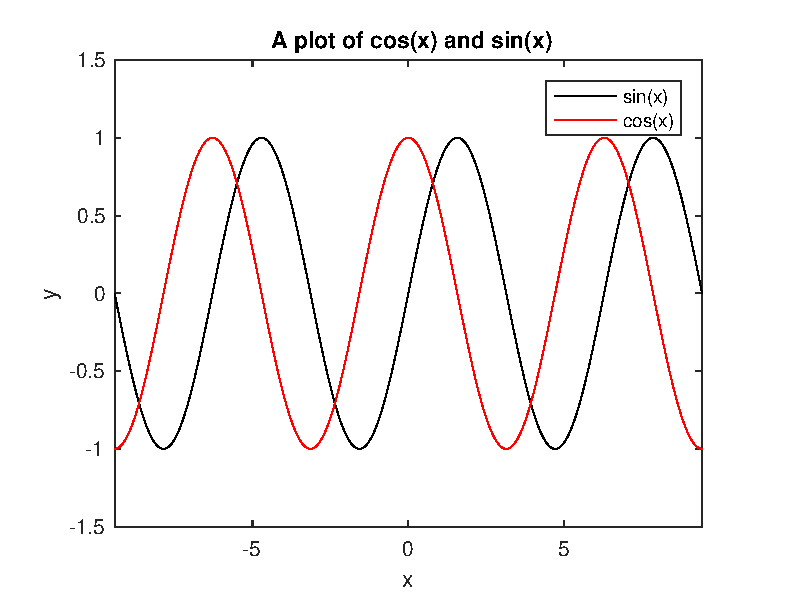
\includegraphics[width=0.4\paperwidth]{plotting.eps}
        \end{exampleBlock}
        
    \end{multicols}
    
\end{document}